\chapter{Introduction}
\label{ch:intro}
\fancyhead[L]{Chapter 1. Introduction}
\fancyhead[C]{}
\fancyhead[R]{}
\fancyfoot[C]{\thepage}

\section{Motivation}
Since ancient times, when peoples like the Olmecs, Chinese and Greeks discovered the strange properties of lodestones \citep{Carlson1975,Evans1977}---magnetic rocks composed of magnetite and hematite---magnetism has marvelled human imagination and been used to aid navigation \citep{May1981}. The fundamental physical theory of magnetism was laid out by the mid nineteenth century \citep{Maxwell1861}; however, understanding of the magnetic properties of rocks would have to wait.\par

In the first half of the twentieth century, systematic studies of how rocks acquire and retain magnetisations \citep{Koenigsberger1938,Thellier1938,Nagata1943} gave rise to the discipline of rock magnetism. Knowledge of rock magnetism has been behind some of the most significant breakthroughs in our understanding of the workings of our planet, e.g., continental drift. Today, insights gained from rock magnetism are used to study the history of Earth's and planetary magnetic fields (palaeomagnetism) \citep{Dunlop} as well as palaeoclimates (environmental magnetism) \citep{Evans}, among other applications in Earth and planetary science.\par

In environmental magnetism, palaeoclimatic conditions can be ascertained from the abundance of and size distributions of magnetic particles found in, e.g., sediments. The smaller particles are magnetised uniformly, this is the so-called single-domain (SD) state. With increasing particle size, a particle can no longer exist in a SD state; the magnetisation curls to produce a single-vortex (SV) structure \citep{Roberts2017} (Fig. \ref{schematic_domains}). Even larger particles form a multi-domain (MD) structure, i.e., multiple regions each uniformly magnetised along different directions. Each of these domain states has different magnetic properties \citep{Dunlop}; rock magnetic measurements can provide estimates for the abundance and size distributions of magnetic minerals and thus palaeoclimatic information. This magnetic proxy for environmental studies also has applications for hydrocarbon exploration \citep{Emmerton2013B,Abubakar2015}.
\begin{figure}
\centering
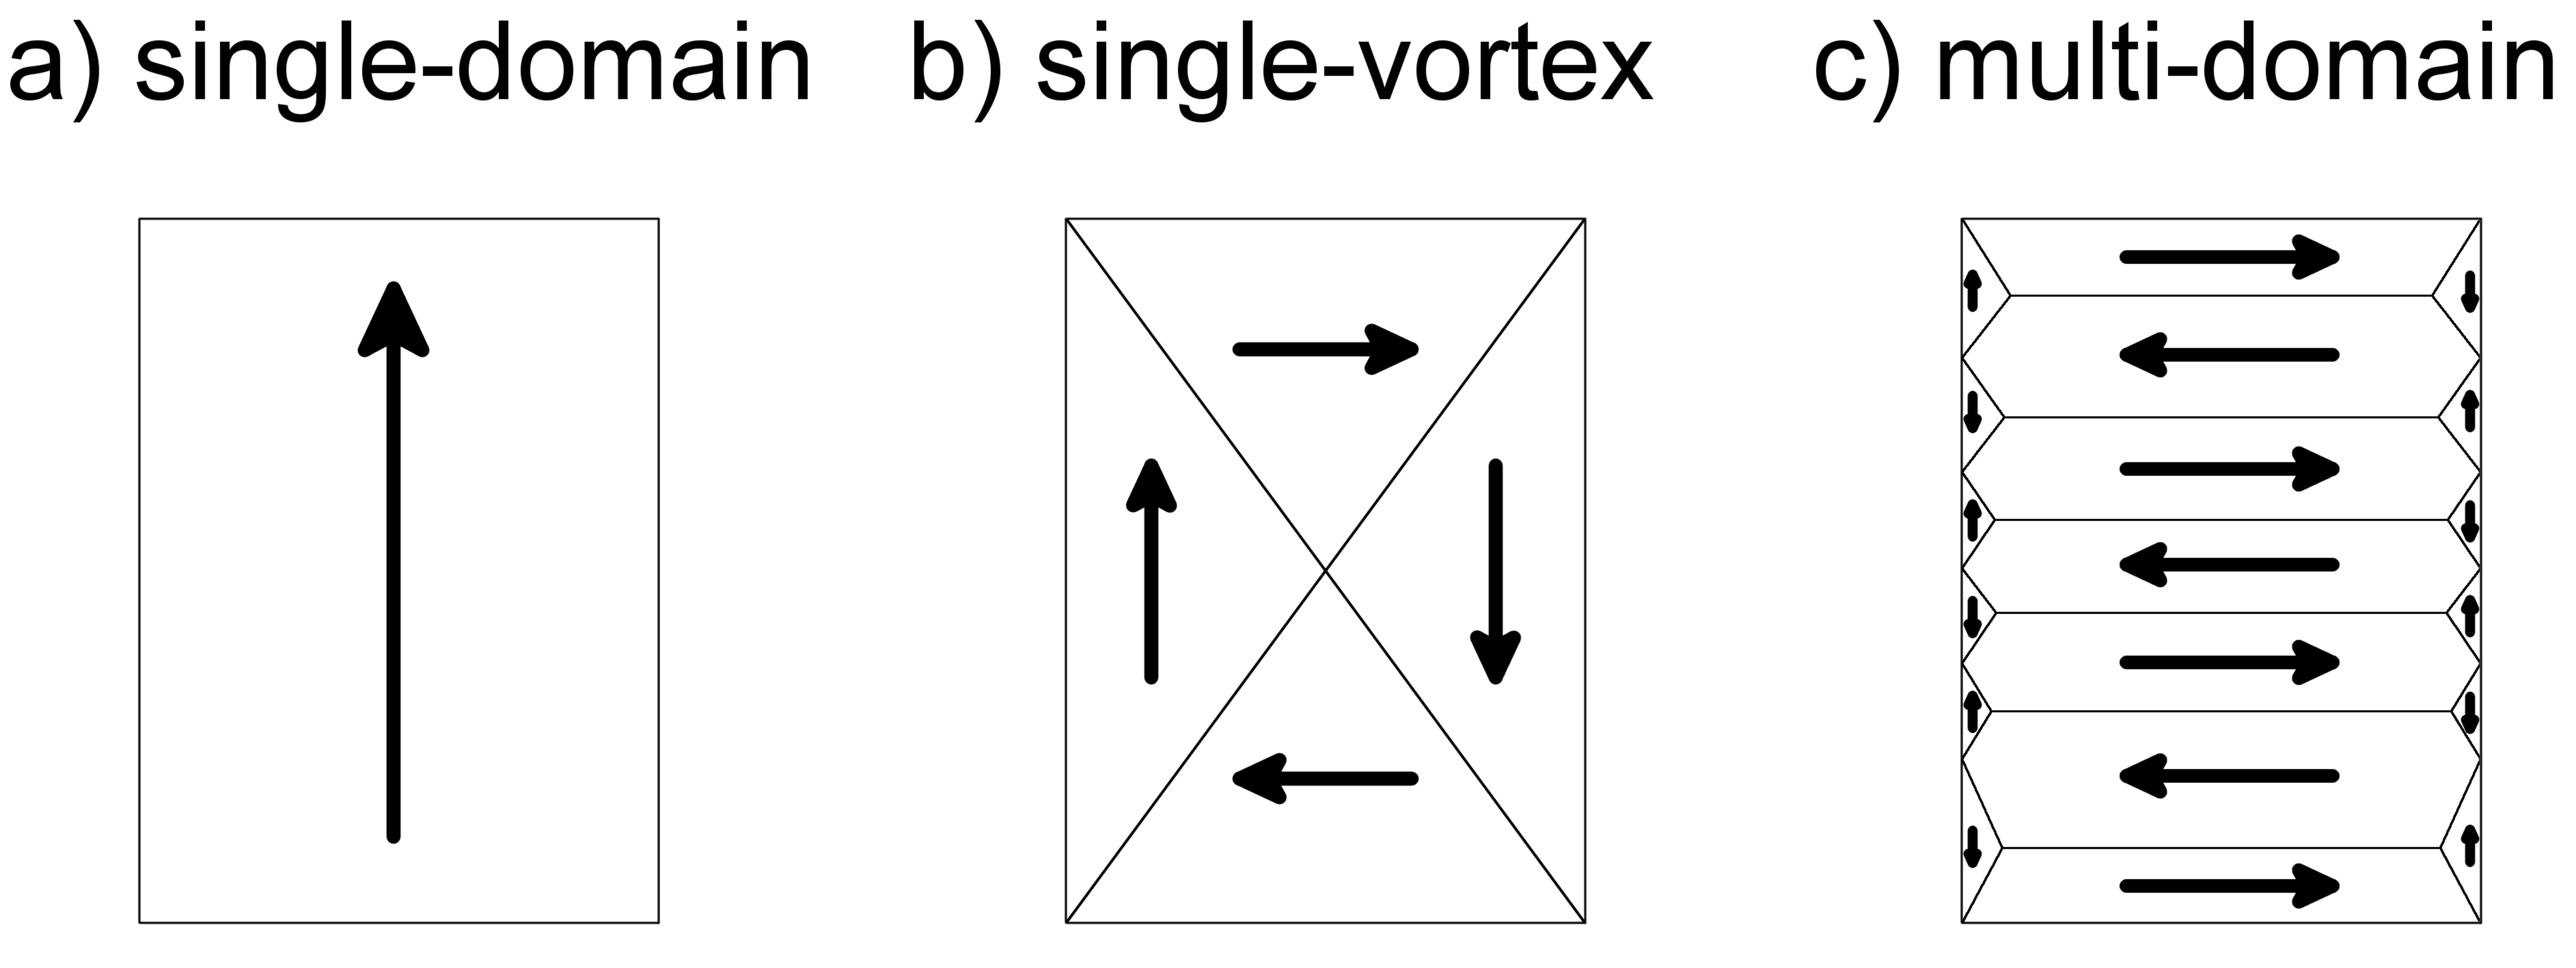
\includegraphics[width=\textwidth]{intro/figs/schematic_domains.pdf}
\caption[Domain state schematic]{Domain state schematic. Single-domain particles (a) are uniformly magnetised (highest magnetic moment). With increasing size, the magnetisation curls into a single-vortex state (b) (lower magnetic moment). In larger particles, the magnetisation is arranged in a multi-domain state (c) with regions called magnetic domains uniformly magnetised (lowest magnetic moment).}
\label{schematic_domains}
\end{figure}\par

Airborne magnetic surveys over oil fields \citep{Donovan1979} have revealed magnetic anomalies, i.e., measurable variations in the background magnetic field. \citet{Donovan1979} suggested that these anomalies are caused by the creation of authigenic near-surface magnetite in an environment of hydrocarbon seepage from the underlying reservoir. Further studies by \citet{Donovan1984}, \citet{Elmore1993} and \citet{Reynolds1993} in the U.S.A., \citet{Diaz2000}, \citet{Costanzo2006,Costanzo2012}, \citet{Gonzalez2002}, \citet{Guzman2011} in Venezuela and \citet{Liu1999}, \citet{Liu2004,Liu2006} in China have provided strong evidence for a genetic relationship between the magnetic contrasts produced by ferrimagnetic minerals near the surface and the underlying reservoir. These investigations confirm the original hypothesis \citep{Donovan1979} that the reducing environment caused by the upward seepage from the reservoirs is conducive to the formation of magnetic minerals such as magnetite and other iron oxides, greigite and other iron sulphides and depletion of minerals such as hematite \citep{Machel1991}, thus furthering the case for using a combination of aeromagnetic surveying and rock-magnetic measurements of soils and rocks for hydrocarbon prospecting.\par

Authigenic formation of magnetic minerals under hydrocarbon-producing conditions has been confirmed by \citet{Abubakar2015}; however, discussion on the exact mechanism for the formation of these minerals at different depths is ongoing. \citet{Machel1991} have identified two primary agents for the precipitation of magnetic minerals under the influence of hydrocarbon seepage. At higher temperatures and thus greater depths they propose chemical processes as the main factor while at shallower depths and lower temperatures it is argued that microbial sulphate-reducing processes are playing the larger role. \citet{Machel1991} also emphasised the difficulty in linking a magnetic anomaly to a process of hydrocarbon seepage because the precipitation of magnetic minerals can cause positive or negative anomalies---that is, peaks or dips in the geomagnetic field and the magnetic susceptibility of the soils. Nevertheless, careful analysis of the local conditions can result in the successful application of rock-magnetic measurements to hydrocarbon exploration \citep{Donovan1984,Liu2006,Emmerton2013B}. Magnetisation of oil-bearing rocks can also be used to assess the quality of oil \citep{Emmerton2013}. It was recognised by \citet{Reynolds1993} that in some cases iron sulphides are more important to the magnetic contrasts and thus to the identification of prospective oil-producing fields than iron oxides. Particularly, greigite has been identified as an authigenic mineral of the utmost importance \citep{Reynolds1993}.\par

Greigite, first discovered in lacustrine sediments \citep{Skinner1964}, is an iron sulphide (Fe$_3$S$_4$) that can be thought of as the sulphide equivalent of the iron oxide magnetite (Fe$_3$O$_4$) as they have the same crystal structure only with sulphur replacing oxygen. Like magnetite, it is highly magnetic \citep{Li2014}. It is commonly formed authigenically in diagenetic anoxic sulphate-reducing sediments \citep{Roberts2011} as a precursor to pyrite \citep{Berner1984,Hunger2007}. Because of its unstable and precursory nature, its importance as a palaeomagnetic recorder has not been as readily realised as that of magnetite. However, geochemical conditions in sediments that are conducive to the long-term preservation of greigite are not uncommon \citep{Roberts2011,Roberts2015} and so, greigite is an important carrier of natural remanent magnetisation (NRM) in many systems \citep{Reynolds1994,Snowball1997,Ron2007,Roberts2010}.\par

Magnetic mineral grains that are linked to hydrocarbon seepage have sizes $\leq 30 \nm$ and thus generally in the SD range \citep{Liu2006}. In terms of morphology, it has been repeatedly found \citep{Ariztegui1996,Snowball1997,Aldana1999,Rowan2006,Roberts2010,Roberts2015} that equant grains of greigite assemble in raspberry-shaped aggregates (Fig. \ref{intro_01}) called framboids (from the French \textit{framboise} meaning raspberry). Presence of magnetic particle framboidal clusters has been linked to chemical alterations produced by hydrocarbon seepage \citep{Aldana1999} and to palaeoclimatic conditions \citep{Ariztegui1996}.\par

Given the unstable nature of greigite and the difficulties to produce synthetic samples, numerical investigations have the potential to answer important questions about greigite that can have great impact on magnetic hydrocarbon exploration and environmental magnetic studies. It is important that the fundamental magnetic parameters of greigite are precisely known to create accurate numerical models. Fabrication of higly pure synthetic greigite allowed \citet{Chang2008} to measure the saturation magnetisation $M_\text{S}$ and the exchange stiffness constant $A$; \citet{Li2014} improved the measurement of the saturation magnetisation. \citet{Winklhofer2014} measured the first estimates for the magnetocrystalline anisotropy (MCA) constants. These studies allow now for accurate models of greigite magnetisations.
\begin{figure}
\centering
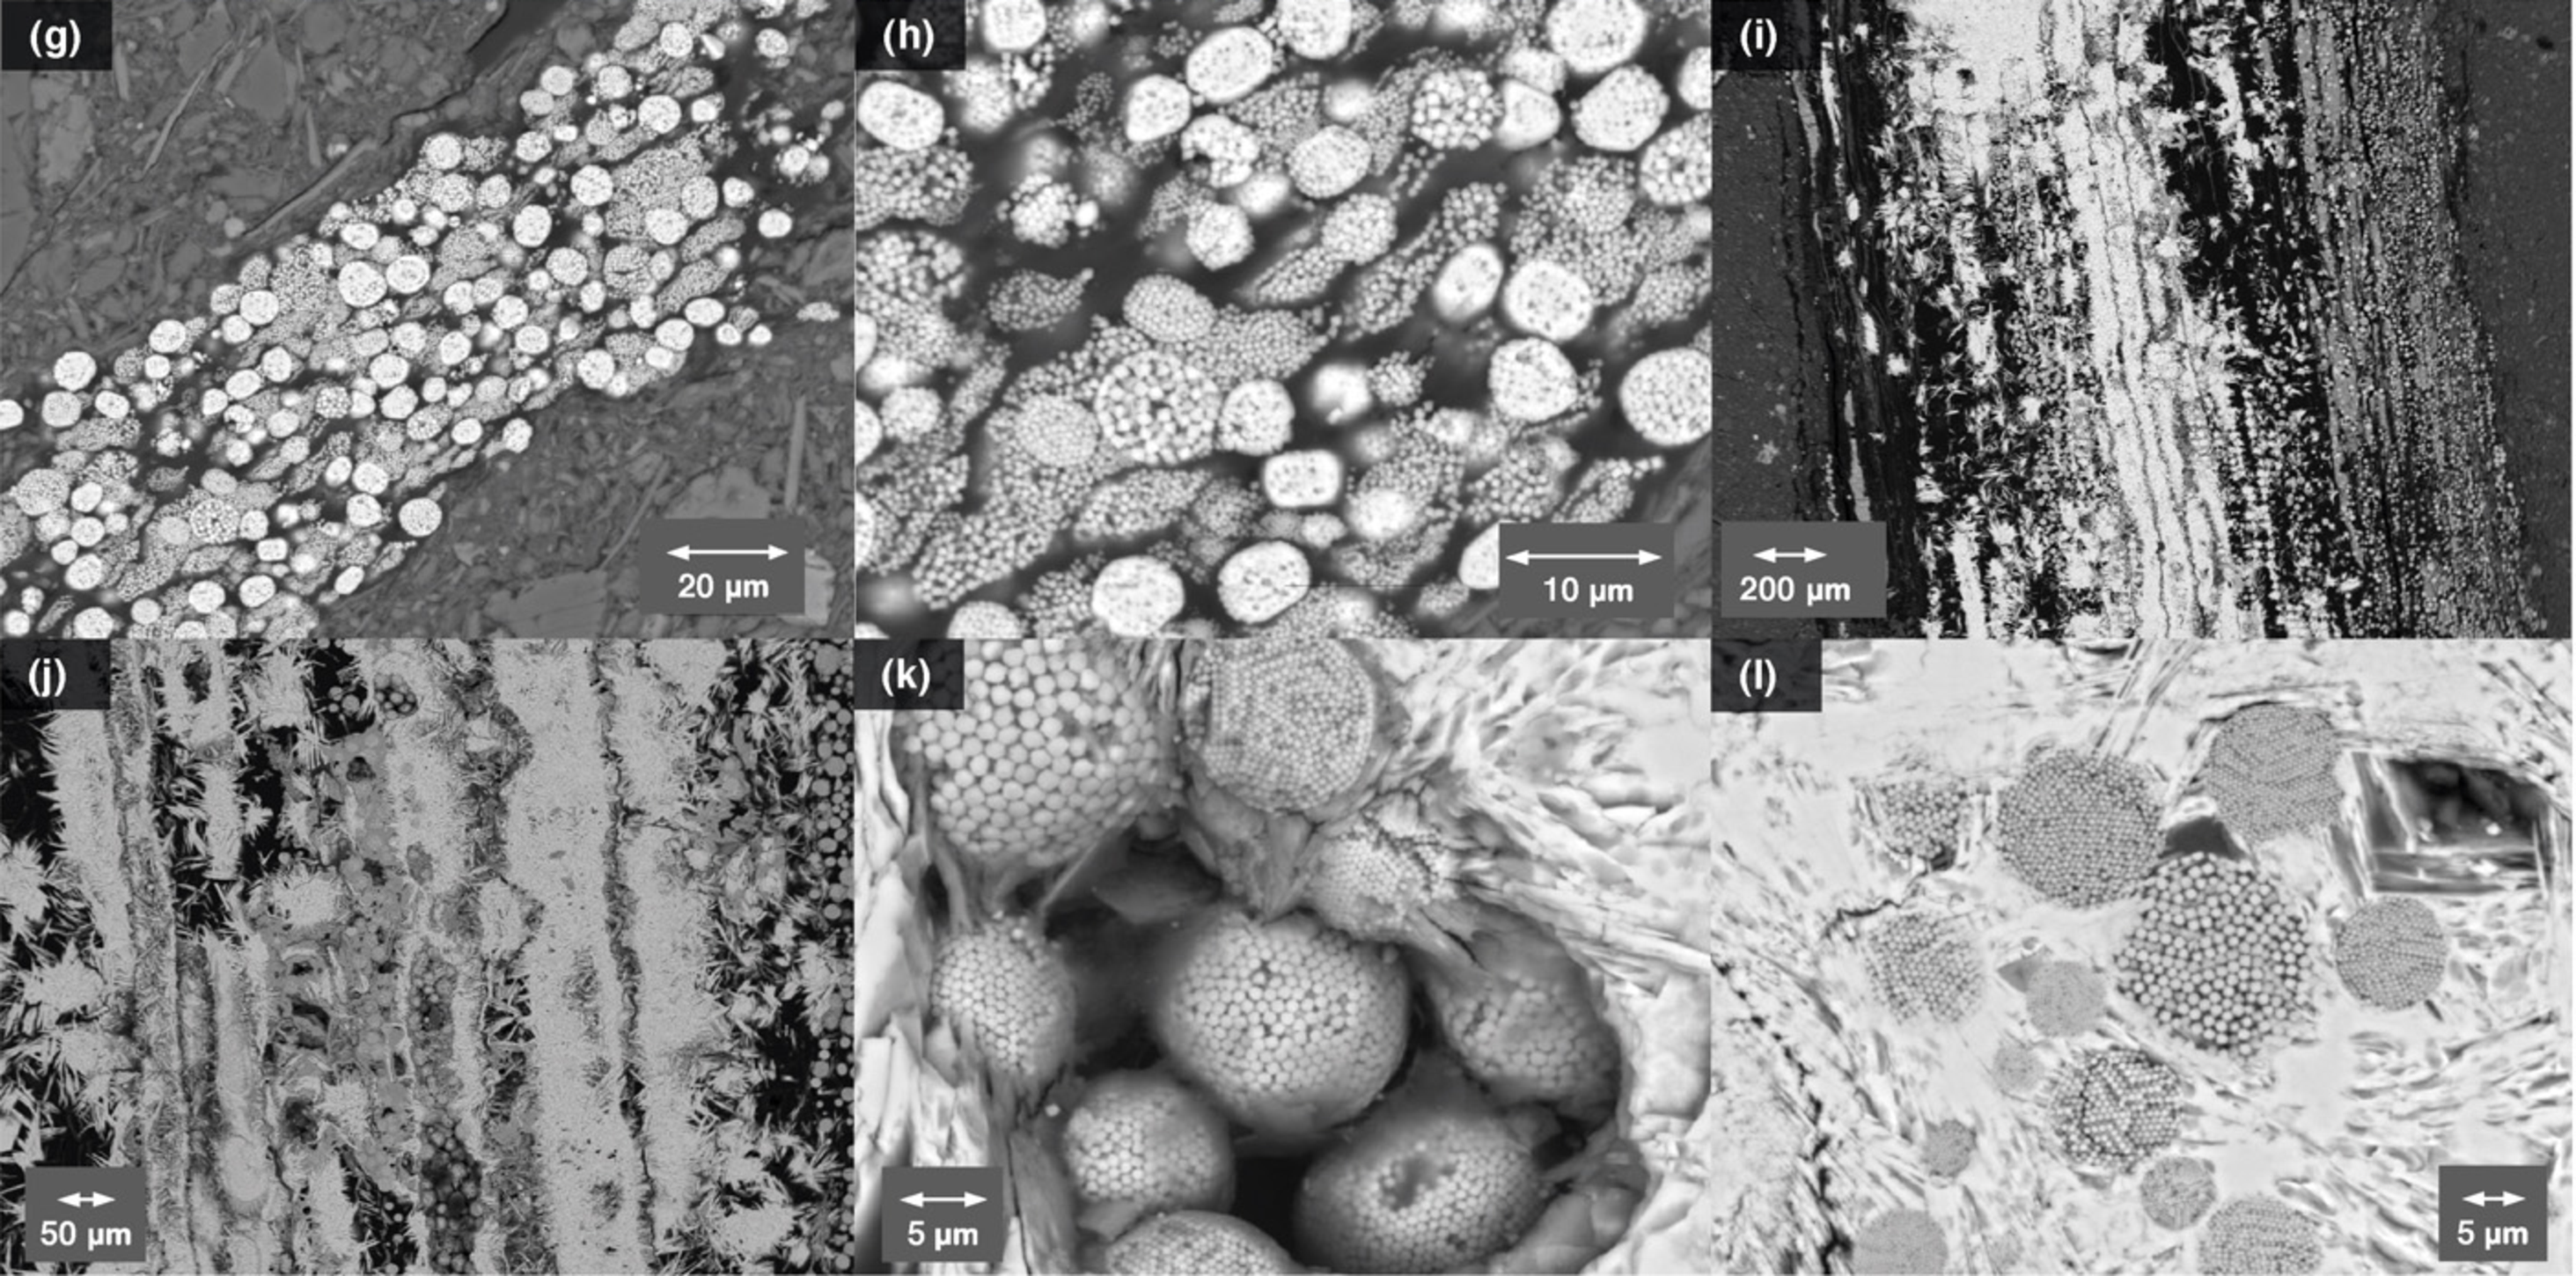
\includegraphics[width=\textwidth]{intro/figs/greigite_framboids.pdf}
\caption[SEM images of framboidal greigite]{Scanning electron microscopy images of iron sulphide minerals. Elongated framboids and non-framboidal pyrite aggregates that probably represent remineralisation of plant cellular matter(g, h). Images at progressively higher magnification of an iron sulphide nodule with evidence of plant matter remineralisation (i--l). The platey minerals are non-magnetic hexagonal pyrrhotite. In (k), a void within the polished surface reveals a cluster of greigite (finest-grained) and pyrite (coarser-grained) framboids that have been overgrown by pyrrhotite (platey texture). (From \citet{Roberts2015}, reproduced with permission from the author).}
\label{intro_01}
\end{figure}
\par

In this thesis, numerical methods are employed to answer some fundamental questions about the magnetic properties of greigite:
\begin{itemize}
\item How does shape and size effect the magnetic structure in sub-micronic greigite?
\item What is the critical size at which greigite can no longer be SD?
\item Can greigite carry stable magnetisations over geological scales?
\end{itemize}
Also, it is important to answer some questions on how these properties effect bulk measurements. In this thesis, the focus is on hysteresis \citep{Mayergoyz1986} and first-order reversal curve (FORC) \citep{Roberts2000} properties:
\begin{itemize}
\item What is the hysteresis and FORC signal of non-interacting SD greigite ensembles?
\item What effect does SV magnetisations have on the non-interacting FORC response?
\item What is the FORC response of framboidal aggregates of greigite?
\end{itemize}\par

\section{The iron sulphide greigite}
\subsection{Greigite occurrence in sediments}
In sulphide-rich sediments, ubiquitous redox reactions cause magnetic iron oxide minerals like magnetite and hematite to be replaced by iron sulphides \citep{Roberts2015}, most commonly pyrite \citep{Berner1984}. Pyrite is a paramagnetic mineral, and thus does not carry a permanent magnetisation. The replacement of magnetite and hematite for pyrite has important consequences for palaeomagnetic analyses of sediments as it can cause the effective destruction of the palaeomagnetic signal \citep{Rowan2009}. This process is pervasive in continental margin marine sediments with high organic carbon contents \citep{Roberts2015}. However, if the rate of Fe$^{2{+}}$ supply exceeds H$_2$S production (e.g. by sulphate-reducing bacteria), iron sulphides that form as precursors to pyrite formation (like greigite) can be preserved \citep{Berner1984}. Greigite can form early during sediment burial \citep{Reynolds1999} or at a later stage, remagnetising the host sediment \citep{Roberts2005} depending on the chronological sequence of the availability of the reactants conducive to greigite preservation. Identification of greigite and the timing of its formation is therefore critical for the magnetic interpretation of sediments.\par

\subsection{Greigite textures: framboidal clusters}
Iron sulphide textures can provide important environmental information about the early sedimentary conditions \citep{Roberts2015}. It is, then, important to identify the texture in which greigite occurs. Among the possible greigite textures, framboidal greigite has been identified as widespread \citep{Ariztegui1996,Wilkin1997} and potentially related to hydrocarbon migration \citep{Aldana1999}.\par

Framboids are spherical aggregates of greigite nano-crystals in which all the crystallites have the same size (Fig. \ref{intro_01}). Greigite and pyrite are often found in framboidal clusters and greigite also filling the space in a less organised manner \citep{Wilkin1997,Roberts2005,Roberts2010,Rowan2006}. Framboid origin is still debated, although some conclusions have been proposed. This morphology does not require biological activity \citep{Sweeney1973,Wilkin1996} although abundance of framboidal greigite is associated with high organic content. It is argued that formation of framboidal greigite is a necessary precursor to pyrite framboids \citep{Sweeney1973,Wilkin1997}. Greigite framboids have been widely observed and the constituent nanocrystals are always finer-grained than neighbouring pyrite crystals \citep{Ariztegui1996,Roberts2005,Roberts2010,Rowan2006}. This is consistent with the pyrite framboid formation process proposed by \citet{Wilkin1997}:
\begin{enumerate}
\item nucleation of iron monosulphide (FeS, mackinawite) nanocrystals,
\item chemical alteration of these into greigite (Fe$_3$S$_4$),
\item aggregation of greigite nanocrystals with uniform sizes to form framboids,
\item replacement of greigite by pyrite (FeS$_2$).
\end{enumerate}
Alternatively, the geochemical balance between iron and sulphur can impede the replacement of greigite by pyrite, leading to greigite preservation.\par

Independently of formation mechanism, an important aspect of greigite and pyrite framboids is that the nanocrystals in all framboids have uniform particle sizes \citep{Wilkin1996}. This is a potential indication that the crystallites nucleated simultaneously, at the same growth rate and thus all under the same geochemical conditions. This is an important observation with potential applications for the timing of sulphidisation events on a geological timescale. Because of this, identification of framboidal greigite is an important problem for environmental magnetic studies. Occurences of magnetite framboids in meteoritic samples have also been observed \citep{Astafieva2004,Kimura2013}; therefore, magnetic mineral framboidal textures are widespread and identification via rock magnetic measurements is an important problem.\par

\subsection{Fundamental magnetic parameters of greigite}
The fundamental magnetic parameters of greigite used throughout this investigation are the saturation magnetisation $M_\text{S}=3.51\,\mu_\text{B}\,\text{p.c.u.}$ \citep{Li2014} or $\roughly 2.7 \times 10^5\,\text{A/m}$  which is $\roughly$11\% higher than the value previously reported by \citet{Chang2009} of $3.25\,\mu_\text{B}$ p.c.u. (and $\roughly$57\% the value of  $M_\text{S}$ for magnetite) and the exchange stiffness constant $A=2\times10^{-12}\,\text{J}/\text{m}$ \citep{Chang2008}. \citet{Winklhofer2014} estimated a cubic MCA constant $K_1=-1.7\times10^4\,\text{J}/\text{m}^3$ and negligible second MCA constant $K_2$ to $K_1$ ratio, i.e., the easy axes are the $<$111$>$, which was confirmed by \citet{Li2014}. Chemical alteration of greigite at high temperatures has made difficult to measure accurately the Curie temperature; however, there is strong evidence for a Curie temperature $T_\text{C}>350\,\text{C}$ \citep{Roberts2010}. In contrast with magnetite, a low-temperature transition has not been observed for greigite \citep{Roberts2010}.\par

\section{Magnetism and matter}
For the purposes of the thesis, a brief review of fundamental concepts of magnetism follows.\par
 
\subsection{Fundamentals of magnetism}
The magnetic induction field $\boldsymbol{B}$, like the electric field $\boldsymbol{E}$, is defined by its effect on a \textit{test particle}, namely, the Lorentz force \citep{Feynman}:
\begin{equation}\label{lorentz}
\boldsymbol{F}_\text{Lorentz} = q(\boldsymbol{E} + \boldsymbol{v}\times\boldsymbol{B}),
\end{equation}
where $q$ is the electrical charge of the test particle and $\boldsymbol{v}$ its velocity. The force a magnetic $\boldsymbol{B}$ field exerts on a moving electrical charge is perpendicular to both its velocity and to the field itself. From Eq. \ref{lorentz}, the units of $\boldsymbol{B}$ are $\text{N}/(\text{C}\cdot\frac{\text{m}}{\text{s}})$, this physically meaningful unit (one Newton of force per charge of one Coulomb moving at one meter per second) is called Tesla, with symbol $\text{T}$.\par

When describing magnetic fields, a distinction between the magnetic induction $\boldsymbol{B}$ and the magnetic field $\boldsymbol{H}$ is made. These denominations, however, are of historical character; it can be proved that the fundamental field is the induction field $\boldsymbol{B}$ \citep{Feynman}. In a vacuum, $\boldsymbol{B}$ and $\boldsymbol{H}$ coincide in direction. In the SI the magnetic and induction fields differ by a scalar factor $\mu_0$, the \textit{magnetic constant}, also known as the vacuum permeability or permeability of free space:
\begin{equation}
\mu_0 = \frac{B_{\text{vacuum}}}{H_{\text{vacuum}}} = 4 \pi \times 10^{-7} \, \text{T}\cdot\frac{\text{m}}{\text{A}}.
\end{equation}
Although the names vacuum permeability and permeability of free space are still widespread it is preferable to use the name magnetic constant since it reflects the fact that it is a defined value and not a measurement.\par

The description of magnetic fields is analogue to that of electrical fields. Although, unlike the situation in electricity, there are no magnetic charges, only magnetic dipoles \citep{Feynman}. The induction due to a wire carrying a current $I$ (generally varying along the path) at a point $\boldsymbol{r}$ can be calculated from the Biot-Savart law:
\begin{equation}
\boldsymbol{B}(\boldsymbol{r}) = \frac{\mu_0}{4\pi} \int_C \frac{I\, \text{d}\boldsymbol{l}\, \times \, \boldsymbol{r}}{r^3},
\end{equation}
where $\text{d}\boldsymbol{l}$ is a differential element of length along the wire in the direction of the current. The integral is carried out along a line, usually but not necessarily a closed curve.\par

In general, it is more interesting and important to consider magnetism in the presence of matter. A material is composed of atoms, which individually may hold a permanent magnetic dipole moment $\boldsymbol{\mu}$ (with units $\text{A}\cdot \text{m}^2$). The \textit{magnetisation} vector field $\boldsymbol{M}$ (with constant norm $|\boldsymbol{M}|=M_\text{S}$) is the spatial average of a myriad of these individual atomic dipole moments over a suitable volume. Therefore, $\boldsymbol{M}$ accounts for the contribution of atomic magnetic moments to the total field. In the SI units we have
\begin{equation}
\boldsymbol{B} = \mu_0 (\boldsymbol{H}+\boldsymbol{M});
\end{equation}
$\boldsymbol{H}$ and $\boldsymbol{M}$ have the same units, the Ampere per meter $\text{A}/\text{m}$. The meaning of this unit is somewhat obscured, but made evident if written in the form $\text{A}/\text{m} = \text{A}\cdot\text{m}^2/\text{m}^3$, i.e., this unit can be thought of as a density of magnetic moments.\par

\subsection{Diamagnetism and paramagnetism}
Magnetism in matter can be broadly categorised into three phenomena: diamagnetism, paramagnetism and ferromagnetism. Diamagnetism and paramagnetism are of little importance to this work so will be only briefly described.\par

Diamagnetism is a property of all matter. It is the smallest effect and is a tendency of a material to oppose an external magnetic field. An external magnetic field exerts a Lorentz force on the bound electrons that causes them to precess like a gyroscope. This is called Larmor precession and is equivalent to an electric current producing a magnetic moment in the direction opposed to the external $\boldsymbol{B}$ field. Water is a common example of a highly diamagnetic material.\par

Paramagnetism is a partial alignment of the atomic magnetic moments of the atoms in a material with an external $\boldsymbol{B}$ field. It is only thermal noise that prevents a perfect alignment of the atomic magnetic moments with the external field, therefore this is a highly temperature dependent phenomenon. Nevertheless, at ordinary temperatures, paramagnetism outweighs diamagnetism by a factor greater than 10.\par

In both diamagnetism and paramagnetism a magnetisation is induced by an external field. The rate at which the magnetisation is acquired with respect to the applied field is called the \textit{magnetic susceptibility} $\chi = \frac{\text{d}\boldsymbol{M}}{\text{d}\boldsymbol{H}}$, in general a tensor.\par

\subsection{Ferromagnetism}
A ferromagnetic material, in contrast with diamagnetic and paramagnetic materials, can retain a (non-saturated) remanent magnetisation in the absence of an external field. In the presence of a relatively weak external field, ferromagnetic materials acquire magnetisations thousands of times stronger than paramagnetic materials. To reconcile these two observations, \cite{Weiss1906} proposed that in ferromagnetic materials there exist magnetic domains, regions which are locally magnetised to saturation, brought about by an \emph{ad-hoc} molecular field; when there is an external field, domains aligned with the field would grow and/or the domains would rotate with the field and when the field is removed the domains would return to random alignments thereby reducing the net magnetisation of the body. Although domain theory was succesful in explaining important aspects of ferromagnetic behaviour, the theory was unsatisfying as it did not explain the origin of the molecular field \citep{Kittel1949}.

Ultimately, ferromagnetism is a phenomenon that cannot be explained solely by classical physics. At the core is the quantum-mechanical concept of exchange coupling, a phenomenon with no classical counterpart \citep{Heisenberg1926}. The origin of ferromagnetism is the alignment of atomic moments (electron spins) by quantum exchange forces. However, in a narrower sense, ferromagnetic materials are those in which \emph{all} the atomic moments share the same alignment. There is a class of materials in which the quantum exchange forces create anti-parallel alignments between atomic moments in different sublattices. When the net magnetic moment of one sublattice is smaller than that of the other, there remains a net moment: these are the ferrimagnetic materials. When the magnetic moments of the different sublattices cancel there is no net magnetic moment: these are the antiferromagnetic materials. Throughout the thesis, the term ferromagnetism is used in a broad sense to include ferrimagnetic behaviour.\par

Exchange coupling is hindered by thermal noise, i.e., ferromagnetic behaviour weakens with increasing temperature. There is a threshold temperature beyond which thermal fluctuations destroy all magnetic ordering and the material becomes paramagnetic; this is the Curie temperature $T_\text{C}$, characteristic of a ferromagnetic material.\par

\citet{Landau1935} obtained a continuum expression for the exchange energy. The main result in \citet{Landau1935} was the theoretical proof that inside a ferromagnetic material there are regions that are magnetised to saturation: the magnetic domains, and that between these domains exist regions where the magnetisation continuously rotates from the direction of one domain to that of the other; these are called \textit{domain walls}. The calculation of \citet{Landau1935} of magnetic domain size and domain wall width and speed of propagation was the first micromagnetic calculation \citep{Brown}.

\section{Micromagnetics}
\citet{Brown} recognised that there was a need for a robust theory on a scale large enough to treat ferromagnetic bodies as a a continuum and small enough to capture the magnetic structure at sub-micron lengths. He called such a theory micromagnetics. The seminal work of \citet{Landau1935} and that of \citet{Brown} are the theoretical basis from which micromagnetics emerged. Micromagnetics is the theory that bridges the fundamental quantum-mechanical picture and the effective macroscopic theory of Maxwell equations. The main goal of micromagnetics is to obtain a configuration of the magnetisation vector $\boldsymbol{M}$ in a ferromagnetic material.\par

\subsection{Magnetic Gibbs free energy}
There are two main approaches to micromagnetism. One is to obtain a configuration of the magnetisation in a ferromagnetic material by minimising the magnetic Gibbs free energy. The other is to solve a partial differential equation (PDE) that describes the dynamics of the magnetic moments; this equation was derived by \citet{Landau1935} and improved by \citet{Gilbert2004} to include damping effects, the Landau-Lifshitz-Gilbert (LLG) equation.\par

It is known from thermodynamics that starting from a nonequilibrium state the evolution of a system can only be such that its Gibbs free energy diminishes. So, by an explicit formulation of the different energies contributing to the total magnetic Gibbs free energy it is possible to find a configuration that is either a local energy minimum (LEM) or global energy minimum (GEM). One of the biggest contributions of micromagnetics to our understanding of magnetic phenomena in matter is that it is quite common for a material to be in a LEM configuration rather than GEM. This is the cause of magnetic hysteresis and magnetic remanence. Disregarding thermal effects and magnetostrictive forces, four magnetic energies contribute to the total. There are microscopic contributions like the exchange energy and the MCA energy. Also macroscopic contributions like the magnetostatic self-energy and the external field energy. The external field is independent of the magnetisation and the exchange and anisotropy energies are short range so these are very easy to calculate. The magnetostatic self-energy, i.e., the interaction between the magnetic moments in the material and the stray field the magnetic body produces is a long range, non-local interaction. This energy creates a demagnetising effect.\par

We can write the total magnetic Gibbs free energy $E_\text{G}$ as the integral of the sum of energy densities $\phi$ associated with these effects \citep{Brown}:
\begin{equation}\label{gibbs0}
E_{\text{G}} = \int_{\Omega} (\phi_{\text{exchange}} + \phi_{\text{anisotropy}} + \phi_{\text{stray}} + \phi_{\text{external}})\, \text{d}^3\boldsymbol{r},
\end{equation}
where $\Omega$ is the ferromagnetic volume and $\text{d}^3\boldsymbol{r}$ the volume differential.\par

The exchange energy is a quantum-mechanical phenomenon wherein the exchange of inner shell electrons between neighbouring atoms results in spin-exchange coupling. The continuum expression was obtained by \citet{Landau1935} and found to be proportional, up to a constant, to the square of the gradient of the magnetisation distribution:
\begin{equation}
\phi_{\text{exchange}} = A | \nabla \boldsymbol{m} |^2,
\end{equation}
where $A$ is the exchange stiffness constant and $\boldsymbol{m}$ is the reduced magnetisation vector, i.e., $\boldsymbol{m}$ is a unit vector in the direction of the magnetisation. This energy density is minimised for uniform magnetisations, therefore, the effect of the exchange energy is to homogenise the distribution of moments.\par

MCA energy is due to the atomic configuration of a crystalline material. The specific arrangement of atoms in the crystal can cause some directions to be easier for the moments to align with \citep{Kittel1949}. These directions are called easy axes. The anisotropy energy of a cubic crystal is given by:
\begin{equation}
\phi_{\text{anisotropy}}=\frac{K_1}{2}\sum_{i\neq j}\gamma_i^2\gamma_j^2 + K_2\prod_i\gamma_i^2,
\end{equation}
where $\gamma_i$ are the magnetisation direction cosines and $K_1$, $K_2$ the first and second anisotropy constants. In terms of the reduced magnetisation vector components, this can be written as:
\begin{equation}
\phi_{\text{anisotropy}}=K_1(m_x^2m_y^2+m_y^2m_z^2+m_z^2m_x^2) + K_2m_x^2m_y^2m_z^2.
\end{equation}
The effect of the MCA energy is a tendency for the magnetic moments to align with the easy axes of magnetisation.\par

The external field energy is the potential energy associated with the interaction of the magnetic moments with an external field:
\begin{equation}
\phi_{\text{external}} = -\boldsymbol{M} \cdot \boldsymbol{B}_{\text{external}},
\end{equation}
where $\boldsymbol{B}_{\text{external}}$ is an external magnetic induction field. This energy tends to align the magnetic moments with the external field.\par

The magnetostatic self-energy is due to the magnetostatic interaction each magnetic moment has with each other. Because in a numerical micromagnetic model there can be hundreds of thousands of individual magnetic moments (mesh/grid points), this is energy is the most numerically expensive to calculate; many methods have been devised to avoid calculating this interaction for each moment, most of these based on the magnetic scalar potential.\par

A partial differential equation for the magnetic potential $\varphi$ is formulated of the form:
\begin{equation}\label{potential}
\nabla^2 \varphi(\boldsymbol{r}) =
\begin{cases}
4\pi\nabla \cdot \boldsymbol{M}, & \text{if }\boldsymbol{r} \in \Omega \\
0,                           & \text{otherwise;}
\end{cases}
\end{equation}
with boundary conditions on the surface $\partial \Omega$:
\begin{align}
\left. \left[ \varphi \right]\right|_{\partial \Omega} &= 0, \\
\left. \left[ \frac{\partial \varphi}{\partial \boldsymbol{\hat{n}}} \right]\right|_{\partial \Omega} &= -4\pi \boldsymbol{M} \cdot \boldsymbol{\hat{n}},
\end{align}
where $\left. \left[\cdots \right]\right|_{\partial \Omega}$ denotes a discontinuity across the boundary (surface) and $\boldsymbol{\hat{n}}$ an outward-pointing surface-normal unit vector. Also, a condition:
\begin{equation}\label{boundary}
\lim_{|\boldsymbol{r}| \to \infty} \varphi(\boldsymbol{r}) = 0
\end{equation}
must be met. Solving this sytem for $\varphi$ is sufficient to calculate the stray field from:
\begin{equation}
\boldsymbol{B}_\text{stray} = -\mu_0 \nabla \varphi.
\end{equation}\par

One of the principal difficulties in solving Eq. \ref{potential} is the limit condition (Eq. \ref{boundary}) because in numerical calculations it is impossible to formally evaluate the potential at infinity. \citet{Imhoff1990} proposed a transformation method that requires space surrounding the ferromagnetic body to be meshed into two concentric shells. The potential is mapped on the outer shell to infinity to satisfy the boundary conditions. A hybrid finite-element method (FEM) and boundary-element method (BEM) formulation \citep{Fredkin1990} does not require free space to be meshed, at the cost of the mathematical complexity involved in the hybrid scheme.\par

The magnetostatic self-energy creates a demagnetising effect, that is, the field $\boldsymbol{B}_{\text{stray}}$ produced by the magnetisation distribution opposes the magnetisation. It is also the phenomenon that has the principal role in the domain structure of large particles. When this demagnetising field is calculated, the magnetostatic self-energy can be expressed as \citep{Brown}:
\begin{equation}
\phi_{\text{stray}} = -\frac{1}{2}\boldsymbol{M}\cdot\boldsymbol{B}_{\text{stray}},
\end{equation}\par
where the factor $1/2$ accounts for the interaction between all magnetic dipoles being counted twice when calculating $\boldsymbol{B}_\text{stray}$.\par

With these expressions for the energy densities, Eq. \ref{gibbs0} can now be rewritten as:
\begin{multline}
E_{\text{G}} = \int_{\Omega} \left( A| \nabla \boldsymbol{m} |^2  + K_1(m_x^2m_y^2+m_y^2m_z^2+m_z^2m_x^2) + K_2m_x^2m_y^2m_z^2 \right. \\
\left. - \boldsymbol{M} \cdot \boldsymbol{B}_{\text{external}} - -\frac{1}{2}\boldsymbol{M}\cdot\boldsymbol{B}_{\text{stray}} \right) \, \text{d}^3\boldsymbol{r}.
\end{multline}
A system out of equilibrium is spontaneously driven to diminish its free energy. The aim of a micromagnetic algorithm is to obtain a distribution of the magnetisation in equilibrum. \citet{Fischbacher2017} describes energy minimisation algorithms for the micromagnetic energy functional. \citet{Brown} proposed a variational method based on the variational derivative of the total energy with respect to the magnetisation. In equilibrium, the variation of the free energy vanishes
\begin{equation}
\frac{\delta E_{\text{G}}}{\delta\boldsymbol{m}} = 0.
\end{equation}
This leads to Brown's equation:
\begin{equation}
\boldsymbol{m} \times \left( \frac{2A}{M_\text{S}}\nabla^2\boldsymbol{m} + \boldsymbol{B}_\text{anisotropy} + \boldsymbol{B}_{\text{external}} + \boldsymbol{B}_{\text{stray}} \right) = 0,
\end{equation}
with $\boldsymbol{B}_\text{anisotropy} = \frac{1}{M_\text{S}}(2K_1m_x(1-m_x^2)+2K_2m_y^2m_z^2m_x)\ihat+(2K_1m_y(1-m_y^2)+2K_2m_z^2m_x^2m_y)\jhat+(2K_1m_z(1-m_z^2)+2K_2m_x^2m_y^2m_z)\boldsymbol{\hat{k}}$. This means that in equilibrium the magnetisation is parallel to an effective field:
\begin{equation}
\boldsymbol{B}_{\text{eff}} = \frac{2A}{M_s}\nabla^2\boldsymbol{m} + \boldsymbol{B}_\text{anisotropy} + \boldsymbol{B}_{\text{external}} + \boldsymbol{B}_{\text{stray}}=\mu_0 \boldsymbol{H}_\text{eff},
\end{equation}
and so, the torque (analogue) acting on the magnetic moments vanishes $\boldsymbol{m} \times \boldsymbol{B}_{\text{eff}} = 0$. This is the motivation to use a dynamical equation involving the torques produced by the effective field as an alternative to energy minimisation.\par

\subsection{The Landau-Lifshitz-Gilbert equation}
Finding an equilibrium magnetisation via energy minimisation (Eq. \ref{gibbs0}) may not always result in physically meaningful distributions. This is because in micromagnetic systems, the energy landscape is usually very complicated and contains many local maxima, minima and saddle points. A more physical approach is finding a solution to the dynamical problem. However, this is numerically more expensive than energy minimisation. The motion of a magnetic moment is mainly due to the Larmor precession around its local field. The Gilbert equation \citep{Gilbert2004} describes this precession and considers damping effects with a single damping constant:
\begin{equation}
\frac{\partial \boldsymbol{M}}{\partial t} = -\gamma\boldsymbol{M}\times\boldsymbol{H}_\text{eff} + \alpha\boldsymbol{M}\times\frac{\partial\boldsymbol{M}}{\partial t},
\end{equation}
where $\gamma = 2.210173 \times 10^5 \frac{\text{m}}{\text{A}\cdot\text{s}}$ is the gyromagnetic ratio and $\alpha$ a phenomenological damping parameter, characteristic of the material \citep{Gilbert2004}. An equivalent formulation is the LLG equation:
\begin{equation}
\frac{\partial\boldsymbol{M}}{\partial t} = -\gamma^{'} \boldsymbol{M}\times\boldsymbol{H}_\text{eff} - \frac{\alpha\gamma^{'}}{M_\text{S}} \boldsymbol{M}\times(\boldsymbol{M}\times\boldsymbol{H}_\text{eff}) \, ,
\end{equation}
with $\gamma^{'} = \gamma / (1+\alpha^2)$.

\subsection{Micromagnetic modelling}
Although the fundamentals of micromagnetic theory were laid out, analytical treatment of the micromagnetic equations was limited to simple cases \citep{Landau1935,Brown1940,Kittel1949}. In order to investigate more complex situations it is necessary to turn to approximate methods. Numerical simulations of the micromagnetic equations are, in the most general case, numerically very expensive, specially the calculation of the long-range nonlinear demagnetising energy due to magnetostatic dipolar interactions. This constrained the early numerical investigations to one- or two-dimensional rotations of the dipoles as well as geometries \citep{Brown1965,Labonte1969,Stapper1969,Aharoni1986,Fredkin1987,Zhu1988}. Although useful to probe the stability of ferromagnetic crystals with palaeomagnetic implications \citep{Moskowitz1979,Moon1984,Enkin1987}, these constrained simulations are very limited as there is no doubt that the true nature of spin structures in ferromagnetic crystals is three-dimensional.\par

\citet{Williams1989} conducted the first unconstrained three-dimensional simulations of single magnetite cubic grains, confirming the critical size of single domain magnetite grains using a conjugate gradient method for minimising the energy. Their method consisted in subdividing a cubic ``sample'' of magnetite into further cubes within the exchange length of the material. Inside each of the cubic cells the magnetisation is the average over a very large number of atomic spins and is represented by a magnetic dipole $\boldsymbol{\mu}$ at the center of the cube. The magnitude of all the dipoles is constant but their directions are allowed to vary. Already in a sample divided into $12\times 12\times 12$ cells, a direct calculation of the demagnetising energy needs around 1.5 million interaction calculations per iteration. Rewriting the demagnetising energy in the manner of \citet{Rhodes1954} they were able to reduce the computation significantly and solve for up to $22\times 22\times 22$ subcubes.\par

While the exchange, anisotropy and external field energy are local and easily calculated, it is the nonlocal dipolar magnetostatic interactions that are the principal obstacle in scaling up simulations. Much of the effort in micromagnetic research has been directed towards creating ever more efficient ways to calculate the demagnetising energy. \citet{Fabian1996} and \citet{Wright1997} developed and applied finite difference (FD) methods based on a fast Fourier transform to calculate the demagnetising energy. This, along growing computing capabilities, has allowed micromagnetics to tackle larger, more complex models \citep{Williams1998}. Nevertheless, FD methods restrict the model geometries to cuboid (rectangular prisms more generally) shapes that, while useful, are somewhat unrealistic shapes for most magnetic minerals.\par

FEMs have the advantage of being more flexible in the geometries that can be modelled; in fact, they allow for arbitrary shapes. This is because the spatial domain is discretised into tetrahedral so-called elements to create an unstructured mesh. This advantage comes at the cost of higher mathematical complexity. In FEMs, to solve a PDE, it is transformed to its \emph{weak form}; the weak form is obtained by multiplying the equation by a so-called test function from a suitable function space and integrating the equation via integration by parts. The solution is found in terms of so-called trial functions; in each node $i$ of the mesh the solution $u_i$ is postulated as a linear combination of the trial functions, e.g., $u_i=a_i\varphi_1 + b_i\varphi_2$, usually $\varphi_j$ are linear `hat' functions. Then, an algebraic equation is formed for each node in the mesh to produce a large system of linear equations for the coefficients $a_i,\,b_i$ which is solved by an appropriate numerical method. The geometric flexibility of FEMs allows the modelling of mineral grains with complex morphologies (e.g. \citet{Williams2010}). For producing the FEM tetrahedral meshes, the proprietary software \emph{Trelis} has been used.\par

The capabilities of today's computers allows to simulate not only single grains but clusters of them that interact magnetostatically with each other. This once untractable problem has been proved to be crucial and influence the critical sizes of single domain grains. \citet{Muxworthy2003}, \citet{Muxworthy2004} and \citet{Muxworthy2006} used a FD method and investigated the effect of magnetostatic interactions between magnetite grains. \citet{Muxworthy2013} used the more recently measured \citep{Chang2008} magnetic parameters of highly pure greigite to investigate the intergrain influence in chains of greigite and its implications for magnetosome crystals, i.e., chains biomineralised by magnetotactic bacteria \citep{Lefevre2011}. However, newer, more accurate values of the magnetic parameters of greigite \citep{Li2014} have since become available. These investigations can be furthered by FEM models of more realistic geometries. In this work, micromagnetic simulations have been carried out using the open-source program \emph{MERRILL} \citep{OConbhui2017}.\par

\section{Brief introduction to the thesis}
In Chapter \ref{ch:res-1}, the zero-field size dependence of the magnetic structure of greigite is investigated for a variety of naturally occurring shapes via a micromagnetic FEM. A nudged elastic-band (NEB) method \citep{Fabian2017} is used to calculate minimal action paths between minimal energy states for a variety of shapes and sizes. This allows calculation of the stability of a magnetisation, with implications for palaeomagnetic studies.\par

A simplified numerical model is developed in Chapter \ref{ch:res-2} to study the hysteresis of small greigite grains in a SD state. A spherical magnetic particle is essentially treated as a magnetic dipole; a gradient method is used to find the energy minimum in an applied field. This model is used to study the FORC diagrams produced by randomly oriented dispersions of non-interacting ideal SD greigite (and iron as another relevant application).\par

A micromagnetic model is used to study the FORC response of randomly oriented non-interacting particle dispersions of greigite with a variety of sizes in Chapter \ref{ch:res-3}. The FORC signal of dispersions of particles with non-uniform, vortex magnetisations is investigated. This model results in heuristics for interpretation of FORC signals when the magnetisations are carried by particles in the SV state. For this endeavour, the micromagnetic models were deployed on Imperial College CX1 high-performance cluster (HPC).\par

The effects of strong inter-particle magnetostatic interactions on the FORC response is investigated in Chapter \ref{ch:res-4}. Framboidal geometries are used to study the FORC signal of randomly oriented dispersions of framboidal greigite. The signal is identified with consequences for the interpretation of FORC diagrams of greigite-rich sediments. The heavy computational demands for these simulations were met by deploying the models on Australian National University Terrawulf HPC.\par

%----------------------------------
%\renewcommand\bibname{{References}}
%\bibliographystyle{elsarticle-harv}
%\bibliography{references}

